\documentclass[a4j,twocolumn]{jsarticle}
\usepackage[dvipdfmx]{graphicx}
\usepackage{url}
\usepackage{amsmath}

\setlength{\textheight}{275mm}
\headheight 5mm
\topmargin -30mm
\textwidth 185mm
\oddsidemargin -15mm
\evensidemargin -15mm
\pagestyle{empty}

\begin{document}

\title{Mg-Zn-Y系合金のLPSO構造におけるL12 クラスターと溶質原子ペアの相互作用の第一原理計算}
\author{情報科学科 \hspace{5mm} 27015448 \hspace{5mm} 日山太智}
\date{}
\maketitle

\section{目的}


LPSO(Long Period Stacking Order) 構造をもつ 
Mg は比 降伏強度で超々ジュラルミン (アルミニウム合金) を上回る特 性を持つため
次世代の航空機の構造材料として注目を集めている.
しかし,LPSO 構造の生成機構は未だ解明されていない.
西谷研究室では
「積層欠陥部に L12 クラスターが形成され,
そこから排斥された Zn, Y が中周期的に濃化して新たな積層欠陥を誘発する」
という溶質原子先導型のシナリオを立て,
Mg-LPSO 合金の溶質原子の単原子構造の計算がおこなわれてきた.

2018年に栃木が行った「溶質原子の単原子構造の長距離位置での計算結果」と「24 層 slab モデ ルでの small cluster と単原子の計算結果の比較」の研究結果から,
図1のように結果は真上方向,第3近接位置ともにほぼ単調な減少を示すというものが得られた.過去の単原子のグラフと比較し,グラフ化したところ近似したグラフが導き出された.
この結果は「中周期的に溶質原子が濃化し,安定する」というシナリオを否定するものとなった\cite{tochigi}.

図2のように2018年に森下がおこなった small cluster を使用した計算結果と比較したところ,
small cluster では最安定値を導き出すことに成功したが,
栃木の研究では,導き出すことはできなかった.
これにより,森下が提唱した「排斥された溶質原子が small cluster を形成し中距離で安定する」という仮説を支持する結果が得られた\cite{donkey}.
しかし,栃木の行った計算は可能性の高いと期待される配置を調べたため,
「溶質原子が単体あるいはペアで中距離で最安定を取る」,あるいは「中距離に規則化する」という作業仮説を完全には棄却するものではない\cite{tochigi}.

本研究では栃木の研究にて取り組んでいない,単原子においての奇数層での第2近接距離で偶数層での第1,第2近接距離での計算,また同条件下においてpairでの計算について検証する.

\begin{figure}[h]
\vspace{0\baselineskip}
\begin{center}
   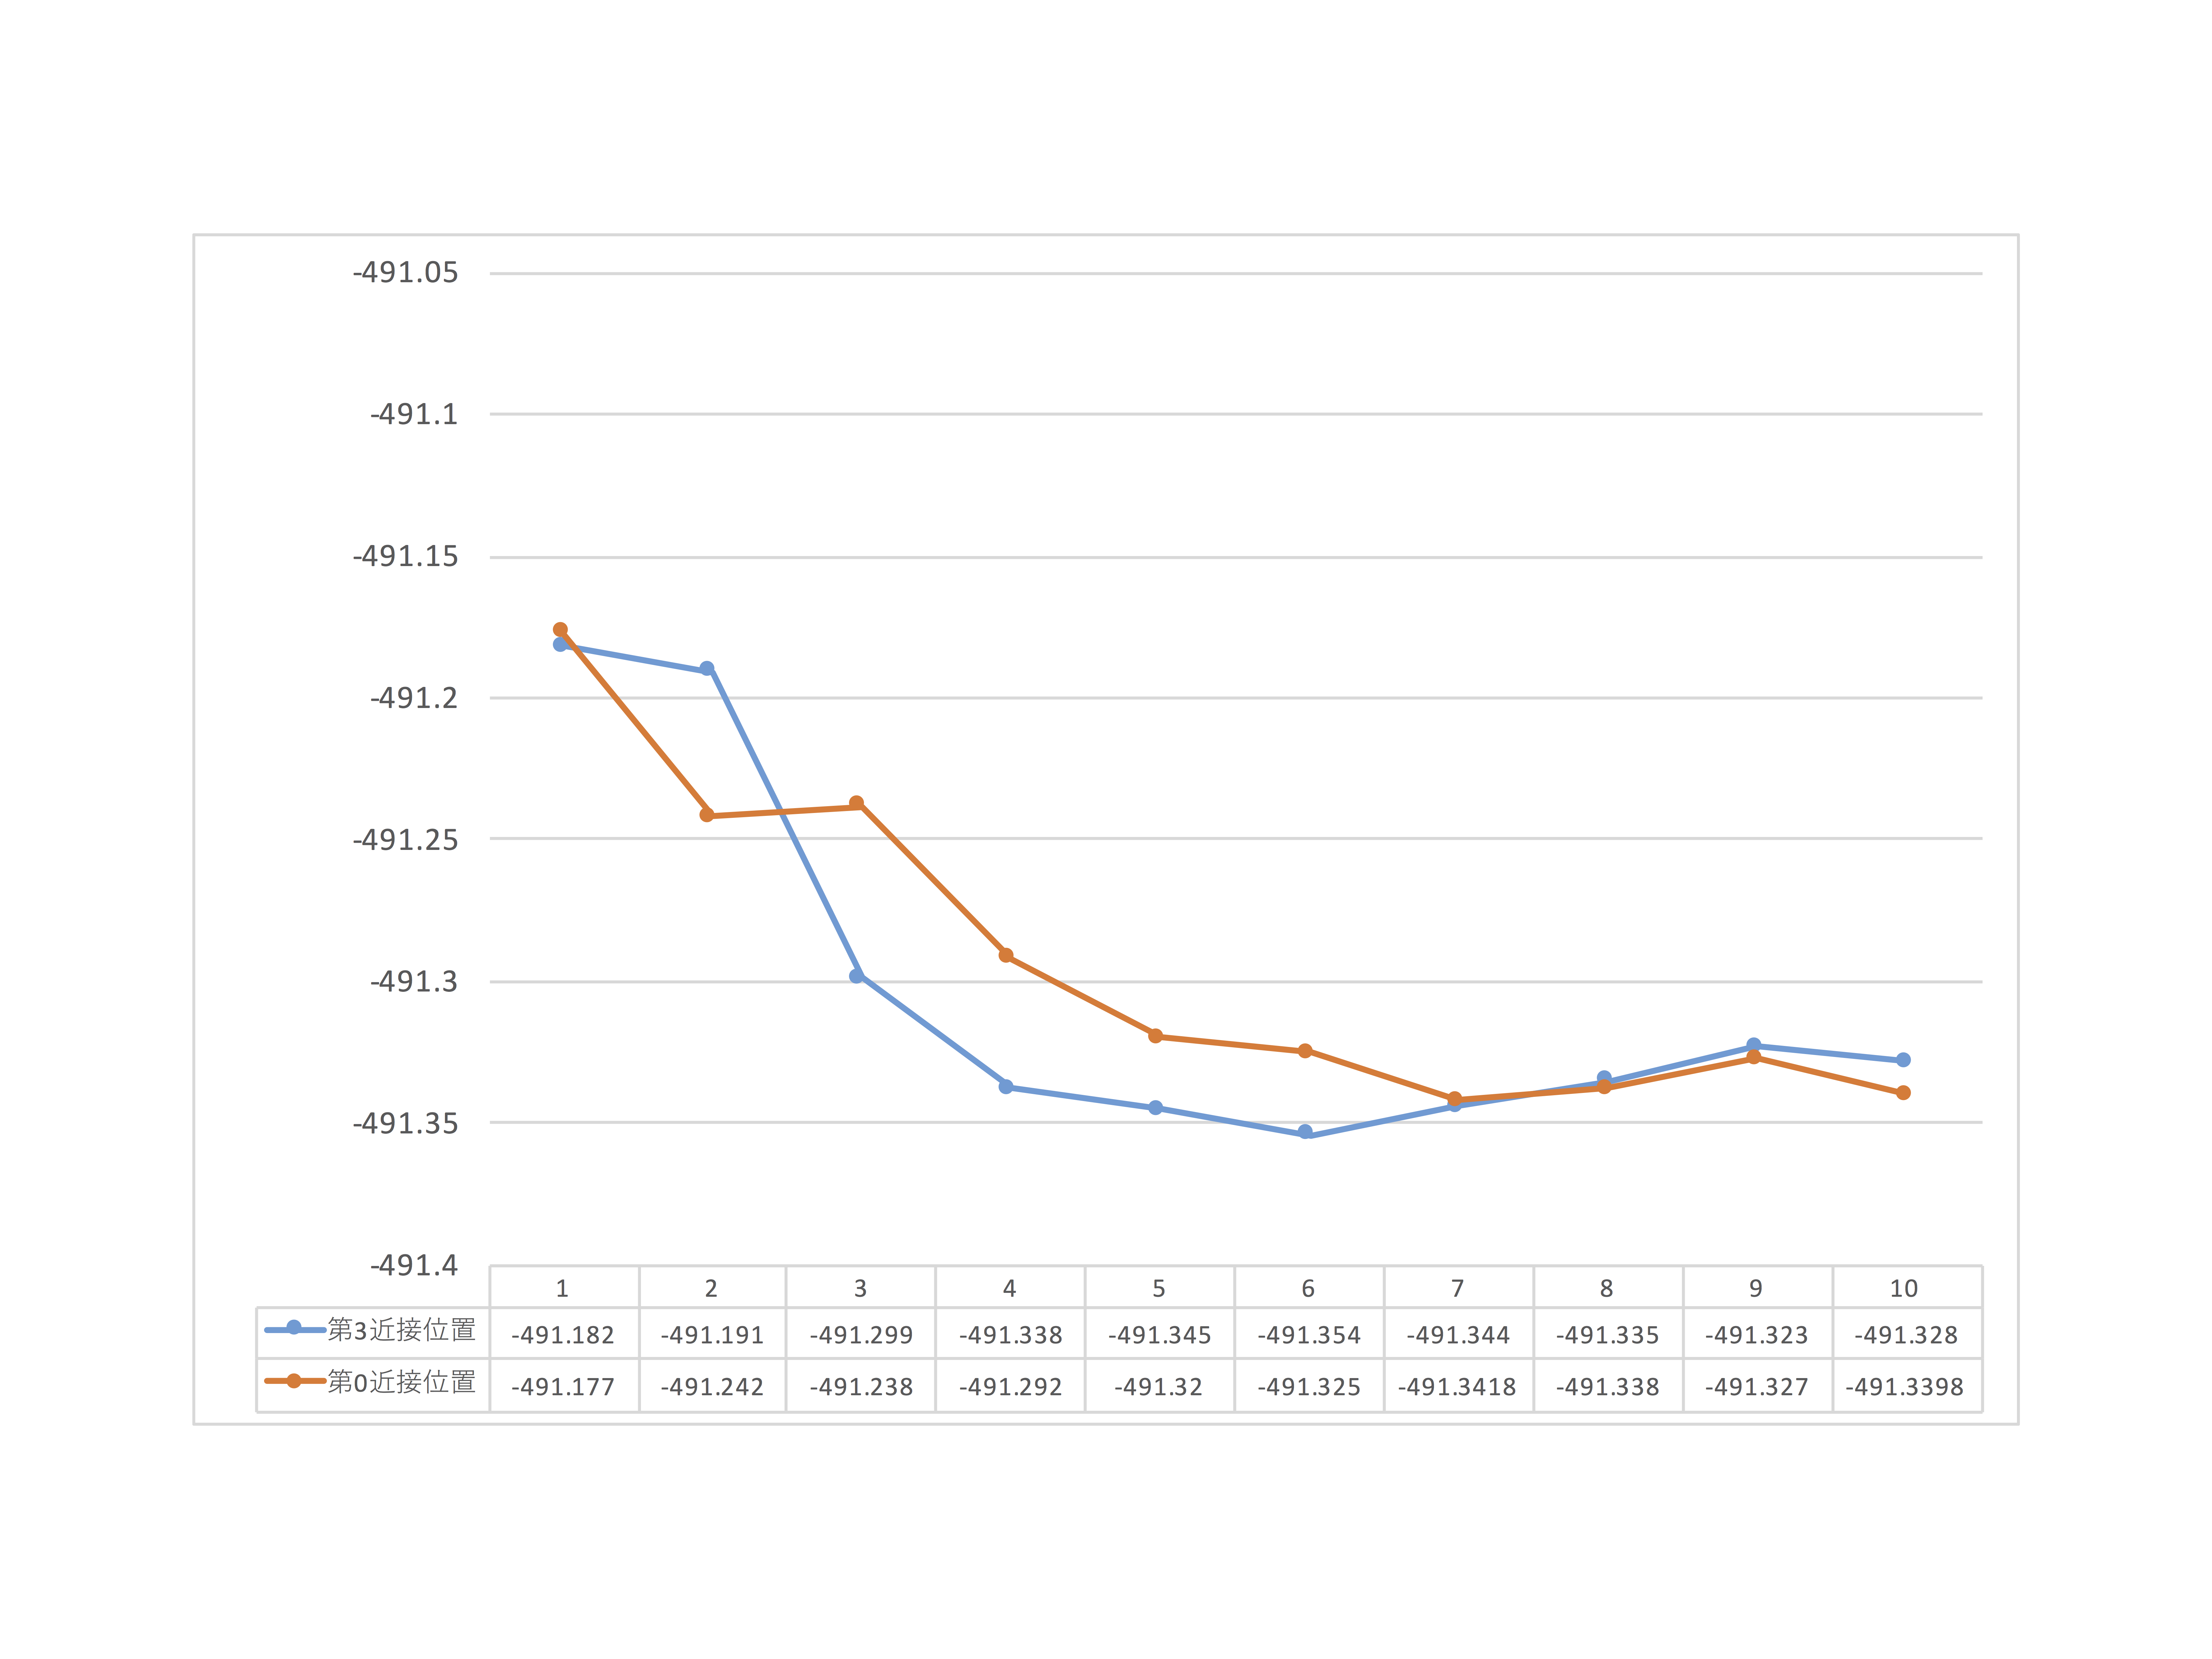
\includegraphics[width=80mm]{../png/0_3garaf.png}
  \caption{第0近接位置と第3近接位置のグラフ結果の比較\cite{tochigi}.\label{glaf}}
  \label{fig:one}
\end{center}
\end{figure}

\begin{figure}[h]
\vspace{0\baselineskip}
\begin{center}
   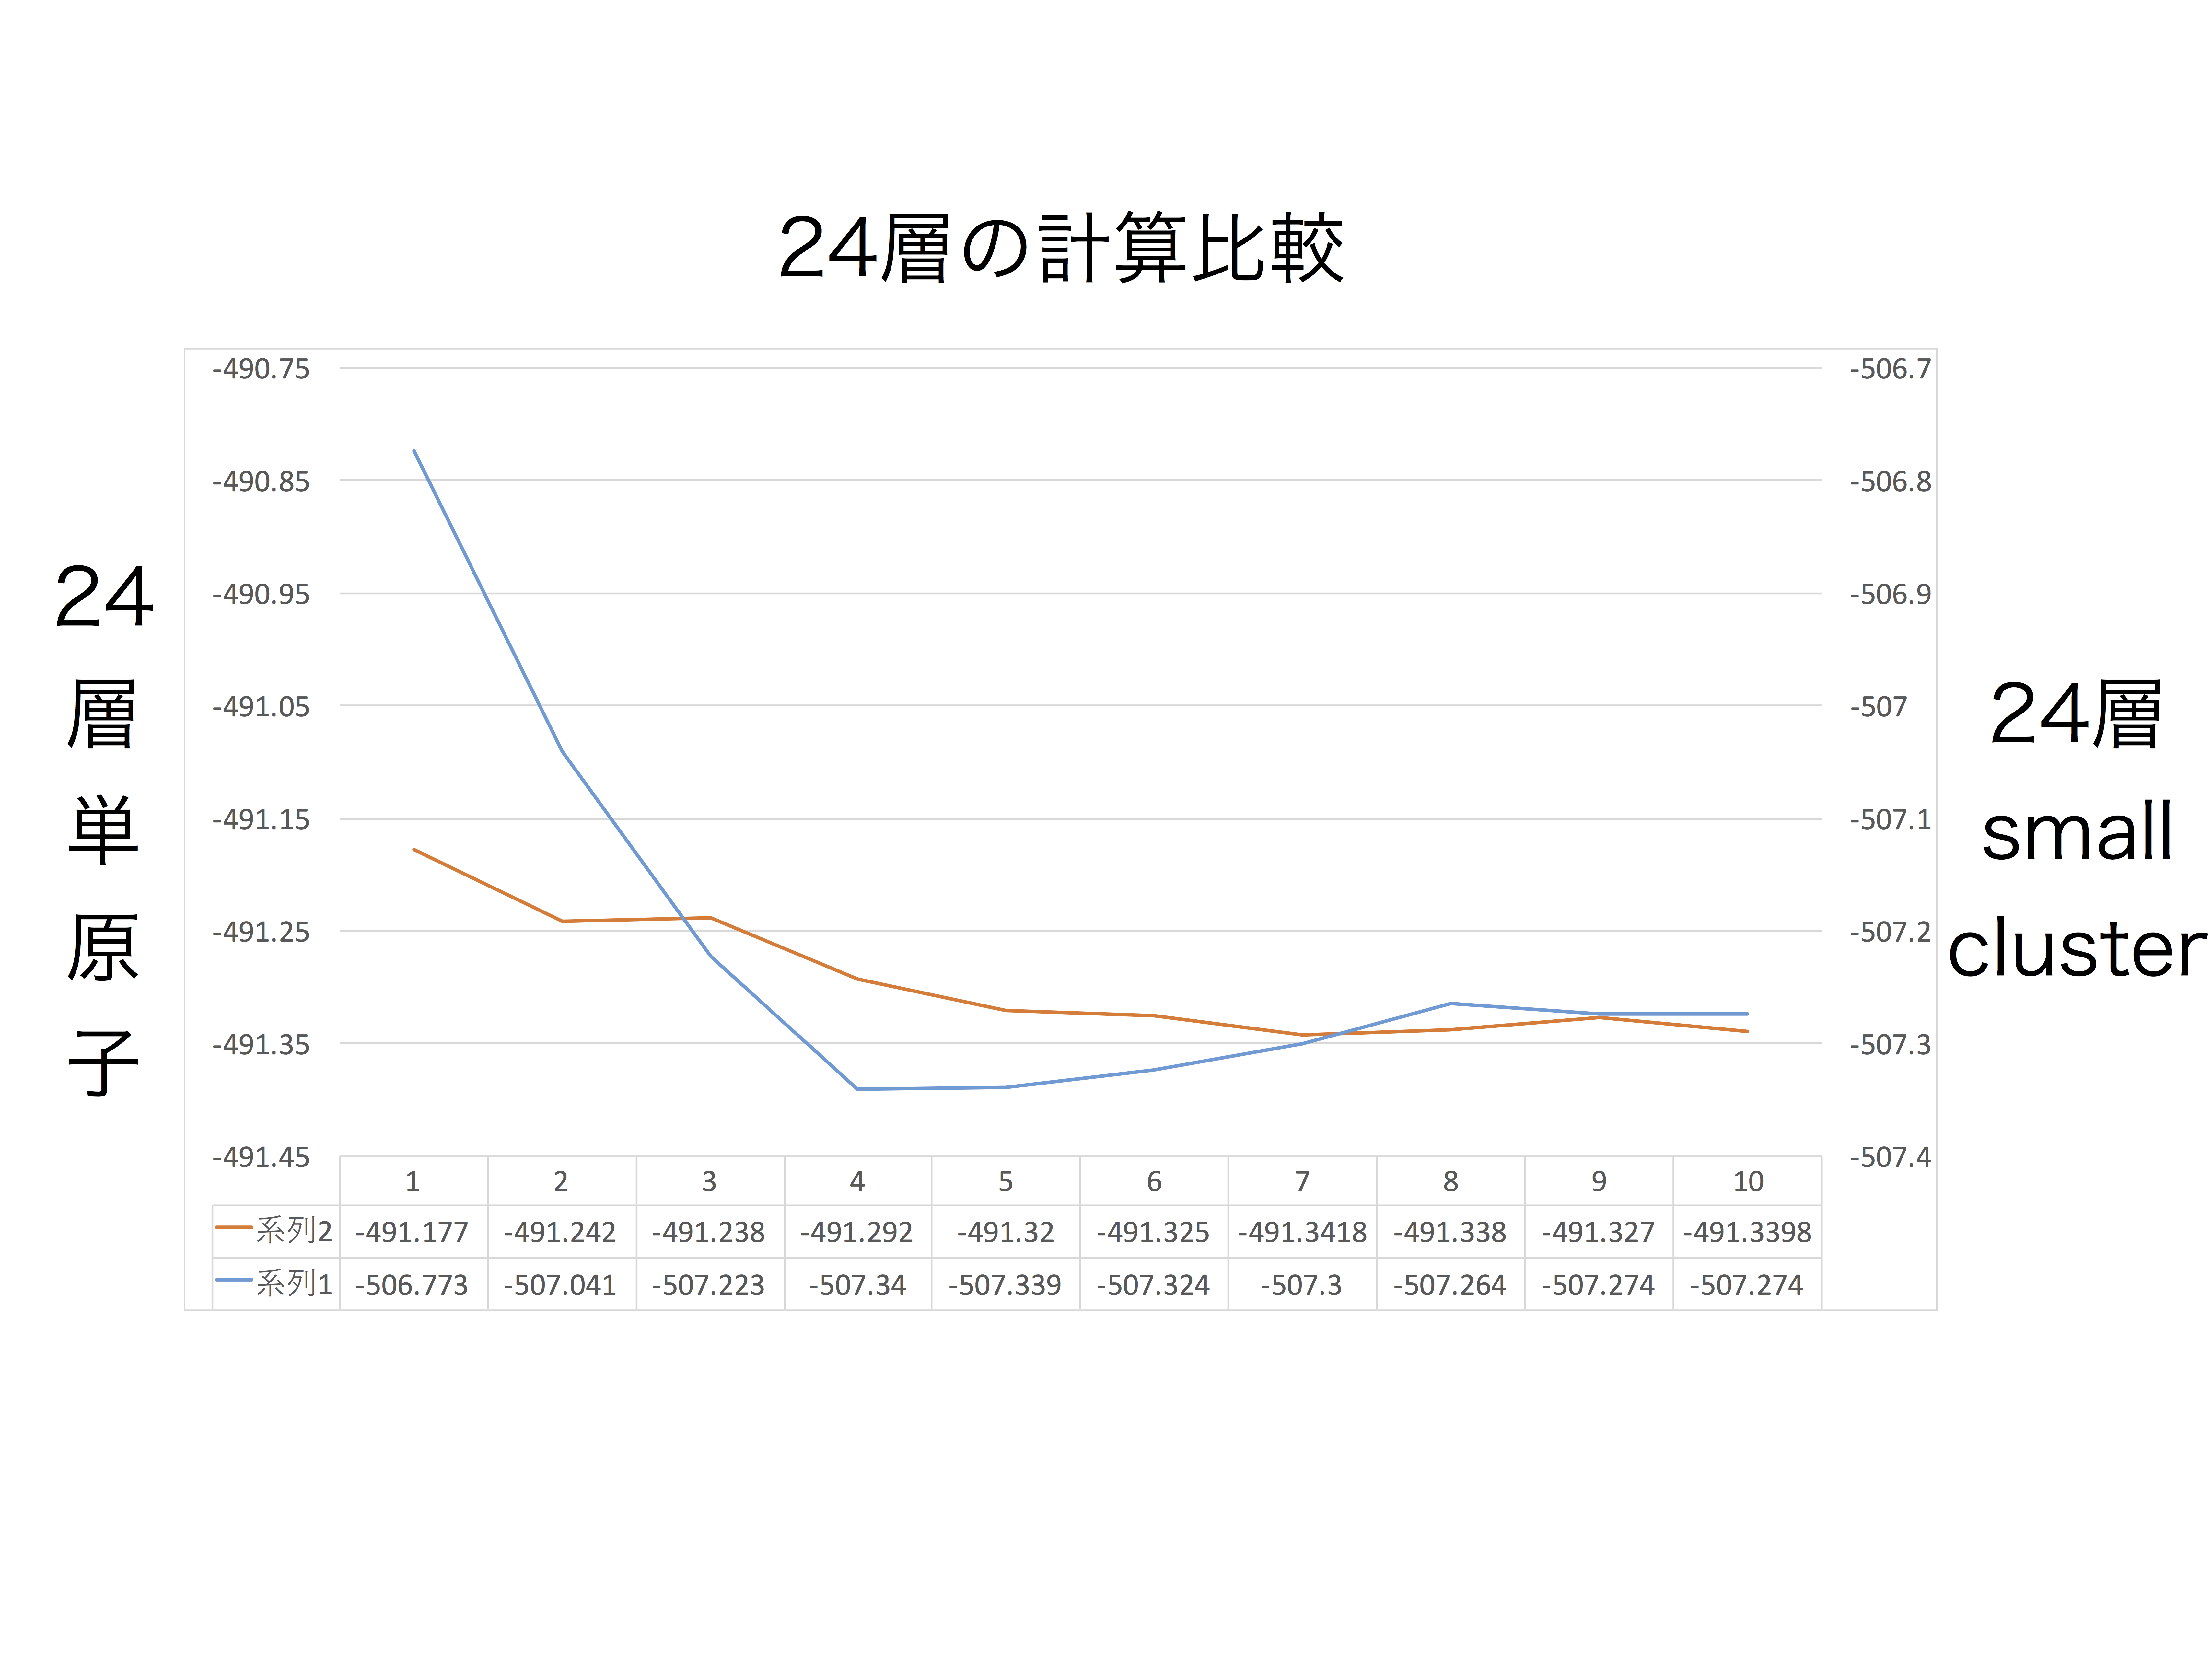
\includegraphics[width=80mm]{../png/24_small_single.png}
  \caption{small cluster と単原子による計算結果\cite{tochigi}. \label{glaf}}
  \label{fig:two}
\end{center}
\end{figure}

\section{手法}

本研究では第一原理計算を行い構造緩和した系全体のエネルギーを求める.第一原理計算はシュレディンガー方程式を解いて,原子の種類だけから精密にエネルギーを求め,様々な物性を予測することができる計算.

また第一原理計算パッケージとして,密度汎関数理論による平面波,擬ポテンシャル法を用いたVASP(Vienna Ab-initio Simulation Package)を用いる.
擬ポテンシャル法とは原子の内殻電子を除いた価電子だけを考慮する手法である.全電子を計算するフルポテンシャル法に比べ比較的高速な計算,また十分な精度を持って計算を行うことができるとされている.

\section{進行状況}
現在,栃木および森下が行った計算を1-layerから順に再度計算をかけて単調減少の傾向を示すのか,また最安定値が導き出るのか確認を行っている.


\vspace{0.5\baselineskip}

{\small\setlength\baselineskip{10pt}	% 参考文献は小さめの文字で行間を詰めてある
\begin{thebibliography}{9}
\bibitem{tochigi}「Mg-LPSO の L12 cluster と溶質原子の長距離相互作用の第一原理計算」 栃木琢治,関西学院大学部論文, (2018).
\bibitem{donkey} 「Mg-Zn-Y 系合金の LPSO 構造における L12 クラスターとスモールクラスターの 相互作用の第一原理計算」森下慎也,関西学院大修士論文,(2018).

\end{thebibliography}
}

\end{document}